\documentclass[11pt, a4paper, oneside]{book}

% Um sprache umzustellen
% \usepackage[ngerman]{babel}
\usepackage[english]{babel}

% Restliche Settings einfügen
\usepackage{Setup/settings}

% Einstellungen für Metainformation in PDF-Datei
\hypersetup{pdftitle={Praktikum Physik 1 Experiment},
            pdfauthor={Till Böhringer}}

% Was im Footer stehen soll, ifoot -> links, cfoot -> mitte
\ifoot{Experiment Shortname}
\cfoot{HS23}

% Allgemeine weite um alle Figures darauf zu beziehen
\newcommand\Plotwidth{0.8}
\newcommand\Bilderwidth{0.8}

\begin{document}

% Bitte Titlepage noch bearbeiten falls nötig
\newgeometry{bottom=1cm, top=4cm} % die Abstände von oben und unten korrigieren
\begin{titlepage}
    \setlength{\headheight}{0cm}
	%\centering
	\includegraphics[width=0.45\textwidth]{\thelogofilename}\par\vspace{1cm}
    % \includesvg[width=0.45\textwidth]{\thelogofilename}\par\vspace{1cm}
	
	\centering
	
	{\bfseries\LARGE University of Zurich\par}
	\vspace{0.7cm}
	
	{\Huge\bfseries Experiment Title\par}
	\vspace{0.7cm}

	{\LARGE Praktikum Physik 1 \par Date of the experiment: DATE \par }
	\vfill

    {\large Author:\par\vspace{0.2cm}}
	{\Large\itshape Till Böhringer\\ \href{mailto:tillnils.boehringer@uzh.ch}{tillnils.boehringer@uzh.ch} \par}
	\vfill

	
	{\large Assistant:\par\vspace{0.2cm}}
	{\Large Dozent McDozentface}
	\vfill
	\vfill

% Bottom of the page
	{\large \today\par}
\end{titlepage}
\restoregeometry % das das restliche Dokument wieder die normale Geometrie hat
\frontmatter

\tableofcontents
\mainmatter

\chapter{Introduction}

In the beginning\cite{Test}...

\begin{figure}[h]
    \centering
    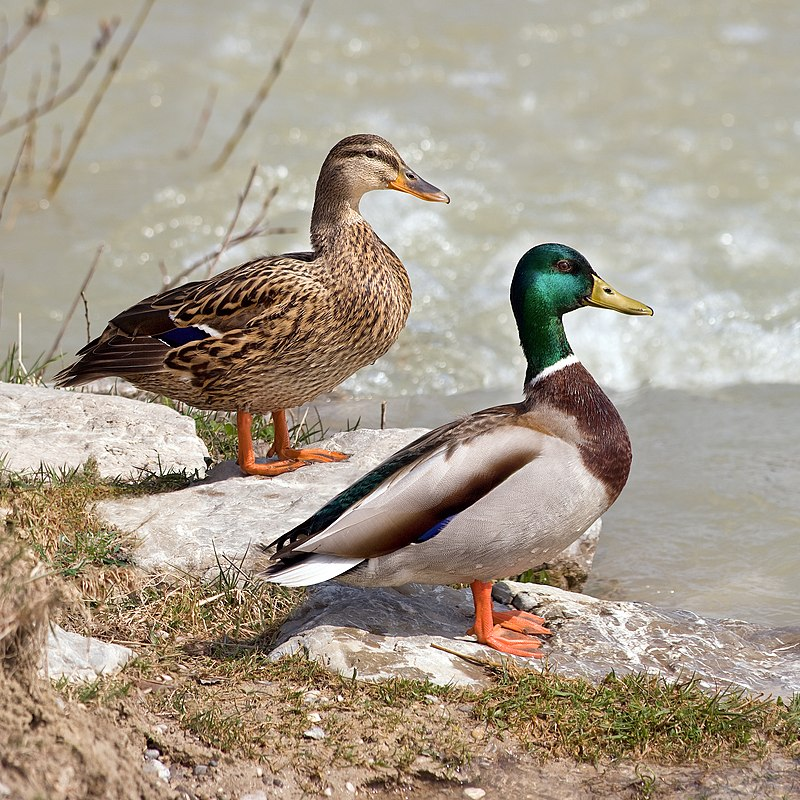
\includegraphics[width=\Bilderwidth\textwidth]{Bilder/example_duck.jpg}
    \caption{Caption}
    \label{fig:Label}
\end{figure}

% \clearpage
% \phantomsection
% \addtocounter{chapter}{1}
% \addcontentsline{toc}{chapter}{\protect\numberline{\thechapter}{\listtablename}}
% \listoftables

% \clearpage
% \phantomsection
% \addtocounter{chapter}{1}
% \addcontentsline{toc}{chapter}{\protect\numberline{\thechapter}{\listfigurename}}
% \listoffigures

% \printbibliography[heading=bibintoc, title={Quellenverzeichnis}]
% \printbibliography[heading=bibintoc]
\IfLanguageName{ngerman}{\printbibliography[heading=bibintoc, title={Quellenverzeichnis}]}{\printbibliography[heading=bibintoc]}

\listoftables

\listoffigures

% \addtocontents{toc}{\protect\newpage}

\end{document}
